\section{范围界定审计协议与实证测试平台}
\label{sec:protocol}

我们依据范围界定综述的 PRISMA 扩展规范（PRISMA-ScR）指南 \cite{tricco2018} 以及经典系统综述方法学 \cite{levac2010} 开展了系统审计。审计协议在全文提取前已预先明确制订，以规范检索字符串、合格性阈值、多轮筛选流程以及评分员间信度消歧。

\subsection{信息来源与文献检索策略}
文献检索覆盖 2023 年 1 月 1 日至 2026 年 3 月 1 日的时间窗口，并滚动监测至 2026 年 7 月以追踪最新预印本。首先，我们通过 OpenAlex API 开展程序化检索（该数据库全面索引 IEEE Xplore、ScienceDirect、SpringerLink、Wiley 与 MDPI）。采用四个题名布尔查询——$Q_1$ (\texttt{"physics-constrained" AND "wind"})、$Q_2$ (\texttt{"physics-informed" AND "wind power"})、$Q_3$ (\texttt{"physics-guided" AND "wind"}) 与 $Q_4$ (\texttt{"physics-embedded" AND "wind power"})——初筛召回 72 项候选记录。其次，针对 Google Scholar、arXiv 与预印本服务器开展靶向检索，补充捕获 17 项在线发表期刊与工作论文，初始候选文献总量达 $N=89$ 项。召回文献与 Scopus 及 IEEE Xplore 进行了交叉核验，以保证对能源与人工智能核心期刊的充分覆盖。全部检索式、原始记录与排除日志均归档于开源补充数据台账中。此外，我们将检索字段拓展至 Scopus 与 IEEE Xplore 题名、摘要与关键词（包含 \texttt{"knowledge-guided"}、\texttt{"hybrid"} 与 \texttt{"domain-informed"} 等更宽泛术语）开展了定向敏感性检索，额外识别出 14 篇文献；全文审查确认其中无一报告失效工况或负面权衡，专门用于压力测试 0.0\% 负面权衡结论的稳健性。需强调的是，这 14 篇敏感性文献专门用于核验负面危害报告；完整的五维（$\mathcal{D}_1$--$\mathcal{D}_5$）深度提取与评分员间信度检验严格在由 PRISMA-ScR 规范确立的核心 46 项研究语料库中开展。

\begin{figure}[!t]
\centering
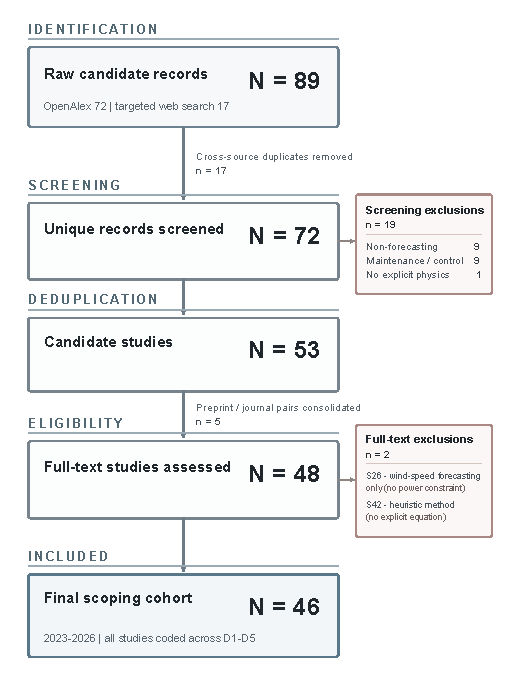
\includegraphics[width=\columnwidth]{prisma_flow_diagram.pdf}
\caption{PRISMA-ScR 范围界定语料库推导流程图 ($89 \rightarrow 72 \rightarrow 53 \rightarrow 48 \rightarrow 46$)。跨源去重消除了17项重复记录，预印本-期刊成对合并去重归并了5项，全文资格审查排除了2项，最终确定 46 项合资格全文研究。}
\label{fig:prisma_flow}
\end{figure}

\subsection{文献筛选、去重与纳入排除准则}
候选记录经历了如图~\ref{fig:prisma_flow}所示的多阶段结构化筛选。跨数据库查重从初始的 89 项记录中剔除了 17 项重复条目，保留 72 项独立记录进入题名与摘要评估。该阶段依据明确标准排除了 19 项记录：9 项聚焦于非预测类任务（如风机结构健康监测、叶片裂纹检测或气弹疲劳损伤建模）；9 项专注于毫秒/秒级实时变桨与有功功率控制而非多步功率预测；1 项不包含任何物理融入建模组件。此阶段最终筛选出 53 项待检索全文的研究。

由于作者在正式期刊录用前通常在公开预印本库（如 arXiv 或 SSRN）发布初稿，将同一课题的预印本与正式期刊论文割裂看待会人为虚增文献统计基数。为此，我们执行了严格的“研究级”（Study-level）成对合并去重准则：只要预印本与已发表同行评审期刊论文共享完全相同的作者群、实证数据集与核心数学公式，两者即被合并为单项研究台账，统一保留正式期刊引用。经过细致比对，共识别并合并了 5 对重复条目（例如 \textit{Applied Energy} 2025 与 SSRN 2024；\textit{Electric Power Systems Research} 2026 与 SSRN 2026），将候选集精炼至 48 项独立研究。

对其余 48 篇全文文献，两名审计员依据三项明确的范围界定合格性准则进行了独立评估：(1) 研究核心聚焦于超短期或短期风电功率预测；(2) 明确形式化构建并在计算中执行了显式物理约束、控制方程或领域边界；(3) 在真实或仿真风电功率时间序列上开展了实证评估。审查最终排除了 2 项研究：研究 S26 仅预测大气风速而未施加风电功率约束；研究 S42 仅实现了启发式特征子空间聚类而无任何领域物理方程。此番严格筛选确立了最终符合 PRISMA-ScR 规范的代表性实证审计文献库，共包含 \textbf{$N=46$ 项独立研究}（涵盖 38 篇同行评审期刊论文与 8 篇具有广泛影响力的预印本/工作论文，包括 UniWind \cite{s27_uniwind2026}）。

\subsection{评分员间信度基准测试}
为在全语料库数据提取前验证 Schema v4 分类体系的操作稳定性，三名独立评分员（Coder A、Coder B 与 Coder C）对分层抽样的 20 篇代表性文献样本进行了双盲独立编码。基准测试显示出各维度高度的评分员间一致性：文献合格性筛选达成百分之百共识（Fleiss $\kappa = 1.000$），精准剔除了对照组 S26 与 S42；参数来源（$\mathcal{D}_1$）在总体与纳入样本上均呈现完美一致性（$\kappa = 1.000$）；作用阶段（$\mathcal{D}_2$）达到近乎完美的一致性（总体 $\kappa = 0.950$，纳入样本 $\kappa = 0.938$）；推理遥测依赖（$\mathcal{D}_3$）呈现出实质性一致（总体 $\kappa = 0.743$，纳入样本 $\kappa = 0.646$）。

相比之下，实现保真度（$\mathcal{D}_4$）在仲裁前的一致性呈现中等水平（总体 $N=20$ 先导样本含负对照时 $\kappa = 0.716$，但严格在纳入样本上时下降至 $\kappa = 0.341$）。这一数值降幅在测量学与统计学中极为典型，反映了著名的 Feinstein 与 Cicchetti 患病率悖论（Prevalence Paradox）：由于纳入样本中高达 92.6\% 的文献未提供公开代码，随机期望一致率极高（$P_e = 86.1\%$），使得即使实际观测一致率高达 $P_o = 90.7\%$，计算出的 Fleiss' $\kappa$ 依然被大幅压低。此外，在缺乏公开代码仓的静态文本阅读中，不同评审员极易对正文宣称的物理约束究竟是“可执行算法”还是“概念性愿景”产生分歧，这一模糊性直接证明了仅凭正文无法可靠推断软件实现，强力支撑了开展底层静态计算图审计的方法学必要性。对于消融语义（$\mathcal{D}_5$），评分员达成高度一致（总体 $\kappa = 0.851$，纳入样本 $\kappa = 0.818$）；而在危害报告方面，三位评分员在 18 篇纳入文献中均一致判定危害报告为零（0/18），由于无边际方差（$P_e = 1.0$），Kappa 统计量在数学上未定义，严格报告为 100\% 观测一致率（$P_o = 1.000$）。在完成先导校准与仲裁一致后，全量 46 篇文献由第一作者（J.L.）完成逐行全文提取并记录精准章节、公式编号与原文证据，并由第二作者（J.D.）对核心定量参数进行独立复核。

\subsection{软件代码审计协议 (PCT 与 PINN-UQ)}
软件可用性审计遵循标准化的五阶段检索流程，全面排查正文主体、脚注、数据与代码可用性声明、出版社公开代码托管库以及作者学术主页。在全量 46 项研究中，仅有两篇论文提供了公开可获取的代码库。其中，PINN-UQ (S10, \textit{Eng. App. AI} 2025) 经审计确认其计算图严格忠实实现了其所陈述的机电代数方程（通过 \texttt{sn.Tie} 实现 $P = g T \omega$ 与 $P = \frac{1}{2} C_p \rho A v^3$），分类为\textit{验证对齐}。另一公开项目物理约束 Transformer (PCT, S02, \textit{Sci. Rep.} 2026) 提供了官方 GitHub 仓库（提交哈希 \texttt{65941ec}），我们对其核心训练脚本（\texttt{train\_clean.py} 和 \texttt{tst/loss.py}）开展了逐行计算图与抽象语法树审计，具体细节见第~\ref{sec:code_audit}节。

\subsection{下游电力系统实际调度与出清结算实证测试基准}
为使实证审计扎根于跨越异质微地形的真实电力系统运行，我们在英国三座商业级陆上风电场（具备10分钟级高精度工业SCADA遥测）上搭建了前瞻性实证测试平台。\textit{Hill of Towie 风电场}（额定装机 48.3~MW，21 台西门子 SWT-2.3-82 机组）地处复杂起伏高地，微地形尾流干扰显著，作为独立时空外推基准（全量 2017 年 7,599 个滚动预报起点，对应 45,594 个下步结算时段），该数据集由 RES 代表 TRIG 在 Zenodo 上以 CC-BY-4.0 许可开源发布 \cite{zenodo_hilloftowie}。\textit{Kelmarsh 风电场}（额定装机 12.3~MW，6 台森吉安 MM92 机组）位于开阔平原农田，作为核心开发基准（8,212 个预报起点，49,272 个结算时段）\cite{zenodo_kelmarsh}。\textit{Penmanshiel 风电场}（额定装机 28.7~MW，14 台森吉安 MM82 机组，编号 WT01--WT15，其中 WT03 缺省）\cite{zenodo_penmanshiel} 位于苏格兰边境丘陵地带，具有 8,440 个预报起点，我们配置了样本受限分区（$N_{\text{train}} = 1,583$），用于测试小样本受限工况下的过拟合与物理先验引导能力。需特别强调的是，由于 Penmanshiel 在地形与机型上与 Kelmarsh 及 Hill of Towie 均存在固有物理差异，跨站点对比必然同时叠加了地形异质性与样本量差异，因此必须依赖场站内受控消融实验以严密隔离样本规模因素。

测试基准在严格冻结的前瞻性协议下运行：输入历史回溯长度 $L=36$（6小时），预测时域 $H=36$（6小时），下游日前调度考核关注次小时交付窗口 $H_{\text{disp}} = \{1, \dots, 6\}$，滚动步长 $S=6$ 以避免相邻结算周期重叠。基准模型套件涵盖无约束 DLinear、边界约束 DLinear ($\lambda=0.01$)、经验功率曲线约束 DLinear ($\lambda=0.01$)、经验条件分布先验 DLinear ($\lambda=0.01$)，并引入经典 Ridge 岭回归与 Persistence 持续性预测作为基准，均在 5 个随机初始化种子下重复评估。此外，为验证发现是否受限于线性结构，我们额外引入了代表性多块通道独立 Transformer 架构（\textbf{PatchTST} \cite{nie2023patchtst}，块长度6，步长4，隐藏维度64，带RevIN的两层编码器），在三座风场、四种约束配置与5个种子下完成 60 次独立训练运行，作为探索性深度架构敏感性基准。

离线决策校准采用后验分位数偏移标定 $\delta_h$，参数严格在独立的 2016 年校准集上拟合（在罚款比率 $r=2$ 下对应临界分位数 $q = 1/(r+1) = 1/3$），对 2017 年测试期 SCADA 与市场价格实现严格盲化。真实市场出清基于英国 Elexon BSC 2017 全年官方系统买入价格（SBP，均值 \pounds 44.27/MWh，峰值 \pounds 1,509.80/MWh，包含 68 个下探至 -\pounds 73.15/MWh 的负电价时段）。结算严格执行 30 分钟物理净偏差结算规则：
\begin{equation}
E_{SP} = \sum_{t \in SP} (p_t - y_t) \cdot \frac{P_{\text{rated}}}{6000} \quad [\text{MWh}],
\label{eq:bsc_netting}
\end{equation}
由此生成单边短缺清算惩罚与双边不平衡结算现金流作为决策风险诊断，所有统计显著性均通过 2,000 次 7 天圆形块成对自举检验（Block Bootstrap）予以严密核验。
